% !TeX spellcheck = es_ES
\chapter{Estado del arte}
\label{ch:chap02}

Este capítulo introduce un resumen de las áreas más importantes relacionadas al trabajo realizado en este proyecto, incluyendo los modelos de iluminación por computadora, el método de radiosidad y sus posibles implementaciones y extensiones.

\section{Modelos de iluminación}
\label{sec:dibujado}

El proceso de dibujado de gráficos tridimensionales por computadora comprende la generación automática de imágenes con cierto nivel de realismo a partir de modelos que componen una \textit{escena} o \textit{mundo} tridimensional, junto a un conjunto de cualidades físicas que rigen las formas en la que la luz interactúa con los objetos.

Este problema puede ser reducido al problema de cálculo del valor de intensidad lumínica observada en un punto $x$ y proveniente directamente de un conjunto de puntos, representado por $x'$. En  \citeyear{Kajiya}, \citeauthor{Kajiya} presentó uno de los modelos más aceptado por la comunidad por su generalidad, la denominada <<ecuación del \textit{rendering}>>:

\begin{equation}
    I(x,x') = g(x,x') \bigg[\epsilon(x,x') + \int_{S} \rho(x,x',x'')I(x',x'') \delta x''\bigg] \label{eq:rendering}
\end{equation}
donde:
\begin{itemize}
    \item $I(x,x')$ describe la intensidad lumínica que llega al punto $x$ proveniente de $x'$.
    \item $g(x,x')$ es un término geométrico, toma el valor de $0$ si existe oclusión entre $x'$ y $x$, y en otro caso su valor es $\dfrac{1}{r^{2}}$ donde $r$ es la distancia entre ambos puntos.
    \item $\epsilon(x,x')$ expresa la intensidad lumínica emitida por la superficie en el punto $x'$ en dirección a $x$.
    \item $\int_{S} \rho(x,x',x'')I(x',x'') \delta x''$ está compuesta por dos términos:
        \begin{itemize}
            \item $\rho(x,x',x'')$ es el término de reflectividad bi-direccional, es decir la proporción de luz que va desde $x''$ a $x$ pasando por $x'$.
            \item $I(x',x'')$ describe la intensidad lumínica observada en el punto $x'$ proveniente de $x''$.
        \end{itemize}
    por lo que este término refiere a la intensidad percibida desde $x$ considerando todas las reflexiones de
    luz posibles para el dominio $S$.
\end{itemize}

Existen distintos métodos de resolución de la ecuación del rendering, donde la mayoría implican cálculos aproximados dado el gran costo de cómputo requerido para hallar una solución exacta. Estos métodos balancean el costo computacional de los algoritmos utilizados y el error del valor obtenido. Existen dos categorías principales para el método: \textit{local} y \textit{global}. Un ejemplo de ambos modelos puede ser observado en la Figura \ref{local-vs-global-img}.

\vspace{5mm}
\begin{figure}[htbp!]
	\begin{subfigure}{0.5\textwidth}
		  	\centering
   		 	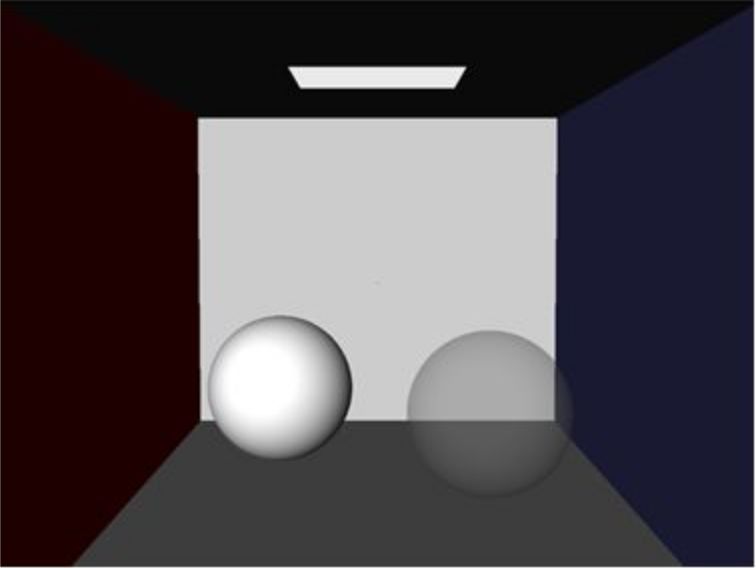
\includegraphics[width=1\linewidth]{assets/local}
   		 	\caption{Local}
   	\end{subfigure}
    \begin{subfigure}{0.5\textwidth}
    	\centering
    	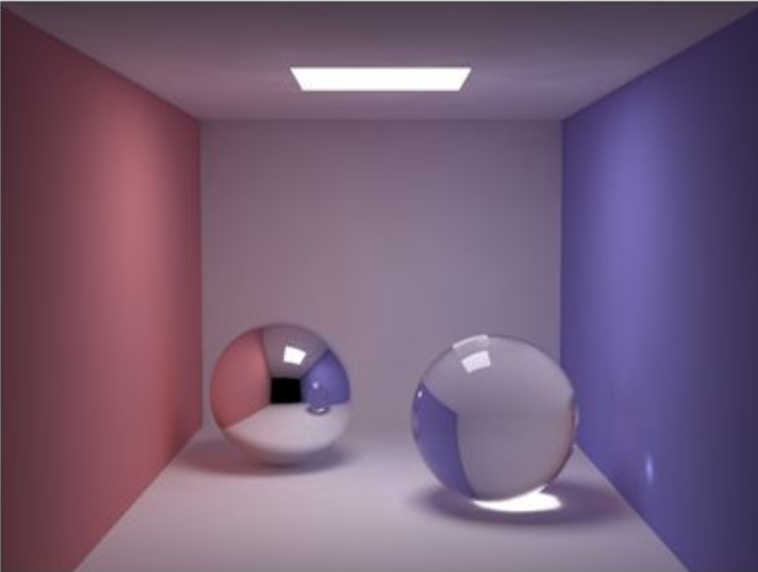
\includegraphics[width=1\linewidth]{assets/global}
    	\caption{Global}
    \end{subfigure}
    \caption{Dibujado utilizando distintos modelos de iluminación.}
    \label{local-vs-global-img}
\end{figure}

\subsection{Iluminación Local}
\label{sec:ilumlocal}
Los modelos de iluminación local tienen en cuenta las propiedades físicas de los materiales
y las superficies de forma individual. Es decir, al dibujar cada objeto no se toman en cuenta las posibles interacciones de los haces de luz con los objetos restantes en la escena. Esto implica que no se proyectan sombras, y tampoco se modelan correctamente las cáusticas producidas por la acumulación de la luz ni el sangrado, entre otros fenómenos de la naturaleza. Estos métodos son más sencillos de implementar y son frecuentemente utilizados en problemas cuya resolución debe ser realizada en tiempo real o por decisiones artísticas.

En referencia a la ecuación del rendering, el término geométrico nunca toma el valor 0, es decir, no se toma en cuenta las colisiones de la luz con otros objetos. El término $\epsilon(x,x')$ toma un valor constante únicamente dependiente de $x$ y $\int_{S} \rho(x,x',x'')I(x',x'') \delta x''$ toma el valor constante $0$.

\subsection{Iluminación Global}
\label{sec:ilumglobal}

El modelo de iluminación global refiere a un conjunto de técnicas que simulan parcial o completamente las interacciones de la luz con todos los objetos que se encuentran  en la escena. Es decir, en contraposición a la iluminación local, se consideran los fenómenos de reflexión y refracción de la luz.

Dependiendo de las característica de los modelos y algoritmos empleados, pueden obtenerse resultados fotorealistas para diferentes escenarios.

El algoritmo de \textit{path-tracing} emula completamente cada haz de luz desde su incepción en una fuente luminosa siguiendo el camino de interacciones del rayo con las distintas superficies de la escena. En este caso el grado de granularidad (que depende directamente de la cantidad de muestras utilizadas) influye en la precisión y calidad en la imagen final. En esencia, el cálculo de la iluminación se basa en un método de Monte Carlo donde para cada punto de la escena se calcula cuánta luz se destina al observador (o cámara) en función de la función de distribución de reflectancia de la superficie como lo sugieren los autores Lafortune y Williams \cite{LW1993BPT}.

Por otro lado, el algoritmo de \textit{mapeado de fotones} propuesto por Jensen \cite{Jensen} supone simular los efectos producidos por las colisiones de las partículas que componen la luz (fotones) con los objetos. Es decir, en la dualidad del modelo de luz onda/partícula supone la segunda interpretación. Las partículas son disparadas desde las fuentes luminosas bajo cierta función de distribución. El algoritmo se compone de dos etapas, en la primera se lanzan los fotones y se construye un mapa de que los relaciona con distintas posiciones de la escena. En la segunda se genera la imagen final a partir de las impresiones que las partículas dejan al interactuar con las superficies de la escena.

Existen además distintas variaciones e híbridos de estos métodos ya que los mismos son demasiado costosos como para dibujar imágenes en tiempo real, en sus versiones originales.

\section{Radiosidad}
\label{sec:radiosidad}

El método de radiosidad es una técnica de iluminación global que emula el transporte de la luz entre superficies difusas. El mismo nombre se utiliza también para describir la magnitud física definida como radiosidad, que indica el flujo de energía radiada por unidad de área ($\frac{W}{m^{2}}$).

Originalmente, este modelo de iluminación global fue propuesto por [\citeauthor{Goral}], y se basa en modelos matemáticos similares a los que resuelven el problema de la transferencia de calor en sistemas cerrados discretos como diferencias finitas o elementos finitos.

\subsection{Radiosidad en superficies lambertianas}

La solución propuesta por \citeauthor{Goral} implica que todas las superficies son idealmente difusas, también conocidas como lambertianas. Estas superficies se comportan como reflectores difusos ideales, lo que significa que reflejan la energía incidente de forma isotrópica siguiendo la regla del coseno como se observa en la Figura \ref{img:lamber}.

\vspace{5mm}
\begin{figure}[h]
	\centering
	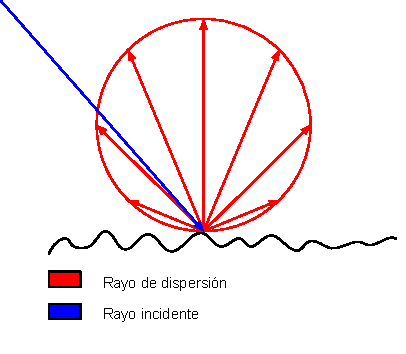
\includegraphics[width=.6\linewidth]{assets/lambert}
	\caption{Reflector lambertiano}
	\label{img:lamber}
\end{figure}

Adicionalmente, se considerará que la energía lumínica irradiada en todas direcciones por cada diferencial de área $\delta_{A}$, puede ser definida como:

\begin{equation}
    I = \frac{\delta{P}}{\cos{\phi\delta\omega}} \label{eq:i}
\end{equation}
donde:
\begin{itemize}
	\item $\omega$ es la dirección de vista.
    \item $I$ es la intensidad de la radiación para un punto de vista particular.
    \item $\delta{P}$ es lae energía de la radiación que emana la superficie en la dirección $\phi$ con ángulo sólido $\delta\omega$.
\end{itemize}

En superficies perfectamente lambertianas, la energía reflejada puede ser expresada como: $\frac{\delta{P}}{\delta{\omega}} = k\cos{\phi}$. Donde $k$ es una constante.
Sustituyendo en \eqref{eq:i} se obtiene: $\frac{\delta{P}}{\delta{\omega}} = \frac{k\cos{\phi}}{\cos{\phi}} = k$, esto implica que la energía percibida de un punto $x$ 
es constante, independientemente del punto de vista.

Es por esto que la energía total que deja una superficie ($P$) puede ser calculada integrando la energía que deja la superficie en cada dirección posible, esto es, se integra la energía saliente en un hemisferio centrado en el punto estudiado:

\begin{equation}
    P = \int_{2\pi} \delta{P} = \int_{2\pi} I\cos{\phi}d{\omega} = I \int_{2\pi} \cos{\phi}d{\omega} = I\pi
    \label{eq:P}
\end{equation}

Por tanto, dada una superficie $S_{i}$, es posible calcular la energía lumínica que deja la superficie utilizando \eqref{eq:P}. Para ello, se discretizan las superficies en parches difusos, lo que transforma la Eq. \eqref{eq:rendering} en:

\begin{equation}
    B_{i} = E_{i} + \rho^{(d)}_{i} \sum_{j=1}^{N} B_{j} F_{ij} \label{eq:radiosity}
\end{equation}
donde:
\begin{itemize}
    \item $B_{i}$ es la intensidad lumínica (radiosidad) que deja la superficie $i$.
    \item $E_{i}$ es la intensidad lumínica directamente emitida por $i$.
    \item $\rho^{(d)}_{i}$ es la reflectividad difusa del material para la superficie $i$.
    \item $F_{ij}$ se denomina \textit{factor de forma}, un término que representa la fracción de energía lumínica va del parche $i$ al parche $j$. 
\end{itemize}

Cabe destacar que la naturaleza recursiva de la ecuación anterior (para calcular $B_{i}$ se debe conocer $B_{j}$) implica que se toman en cuenta todas las reflexiones difusas que existan en la escena. Como se puede observar, resolver el sistema de $N$ ecuaciones lineales bastaría para conocer la energía emitida por cada parche. 

Los factores de emisión y reflexión, para cada parche $i$: $E_{i}$ y $\mathbf{\rho^{(d)}_{i}}$ respectivamente, dependen de los materiales que compongan la escena y son parámetros dados. Sólo resta computar la matriz de factores de forma $\mathbf{F}$ para poder calcular el vector de radiosidades $B$. 

Para determinar una entrada de la matriz $F_{ij}$ involucrando a las superficies $i$ y $j$ de área $A(i)$, $A(j)$, considerando los diferenciales infinitesimales de área $\delta{A_{i}}$, $d{A_{j}}$, representados en la Figura \ref{img:ff2}, el ángulo sólido visto por $d{A_{i}}$ es $d{\omega} = \frac{\cos{\phi_{j}d{A_{j}}}}{r^{2}}$. Sustituyendo en \eqref{eq:P} se obtiene:

\begin{equation}
    d{P}_{i}d{A_{i}} = I_{i} \cos{\phi_{i}}d{\omega}d{A_{i}} = \frac{P_{i}\cos{\phi_{i}}\cos{\phi_{j}}d{A_{i}}d{A_{j}}}{\pi r^{2}}
\end{equation}

\vspace{5mm}
\begin{figure}[htbp]
	\centering
	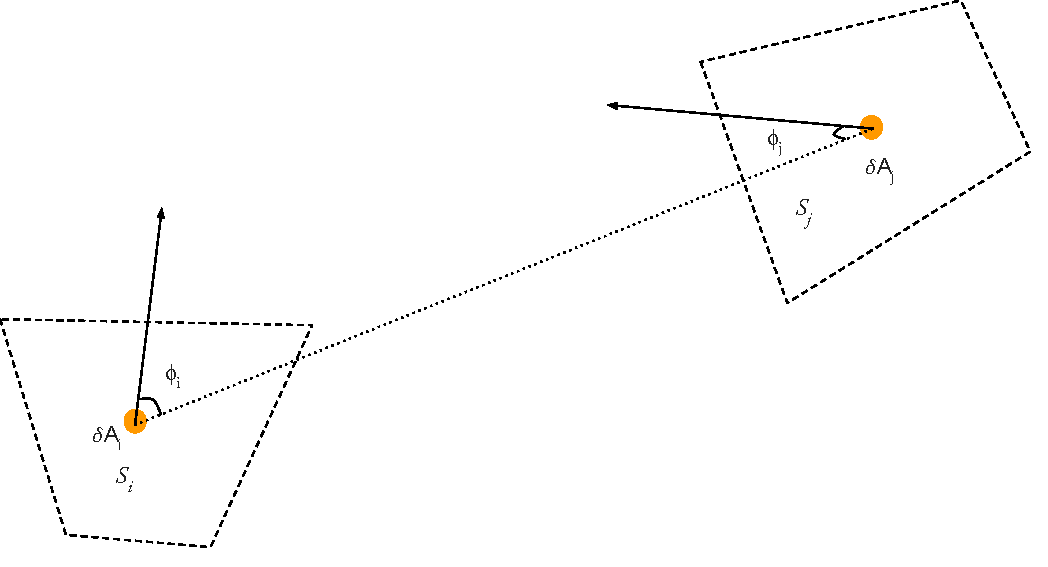
\includegraphics[width=0.8\linewidth]{assets/ff}
	\caption{El factor de forma entre dos superficies}
	\label{img:ff2}
\end{figure}


Considerando que ${P}_{i}{A_{i}}$ es la energía que deja $i$, y que el factor de forma $F_{ij}$ representa la fracción de dicha energía que llega a $j$ podemos observar que:

\begin{equation}
    F_{\delta{A_{i}}-\delta{A_{j}}} = \frac{\cos{\phi_{i}}\cos{\phi_{j}}\delta{A_{j}}}{\pi r^{2}} = \frac{\cos{\phi_{i}}\cos{\phi_{j}}\delta{A_{i}}}{\pi{r^{2}}}
\end{equation}

Integrando, para obtener el factor de forma para el área total:

\begin{equation}
    F_{ij} = \frac{1}{A_{i}} \int_{A_{i}}\int_{A_{j}}\frac{\cos{\phi_{i}}\cos{\phi_{j}}\delta{A_{i}}\delta{A_{j}}}{\pi{r^{2}}} \label{eq:ff}    
\end{equation}

De \eqref{eq:ff} se obtienen las siguientes propiedades:
\begin{enumerate}
	\label{propsff}
    \item $A_{i}F_{ij} = A_{j}F{ij}$, lo que supone una relación simétrica entre los factores de forma.
    \item $\sum_{j=1}^{N} F_{ij} < 1$ Es decir, la suma de una de las filas de la matriz de factores de forma no podrá tener un valor superior a la unidad.
    \item $F_{ii} = 0$ Esto se debe a que los parches considerados son planos y por tanto no reflejan su propia luz.
    \item $F_{ij}$ toma el valor correspondiente a la proyección de $j$ en un hemisferio unitario centrado en $i$, proyectándola a su vez en un disco unitario.
\end{enumerate}


\subsection{Métodos de cálculo de la matriz de Factores de Forma}
\label{sec:calculoff}

El cálculo de los factores de forma a través de la Eq. \eqref{eq:ff} analíticamente es inviable en la práctica pues supone la necesidad de conocer la visibilidad entre cada par de parches que componen la escena. Por tanto, es necesario establecer otros métodos que provean aproximaciones lo suficientemente correctas.

Geométricamente, puede establecerse una analogía para la computación de factores de forma conocida como <<analogía de Nusselt>> (ver Figura \ref{img:nusselt}). Se expresará el factor de forma como la proporción de área proyectada de $S_{j}$ en un hemisferio ubicado en el baricentro de $S_{i}$ y luego en un disco centrado en $S_{i}$.

\begin{figure}[H]
	\centering
	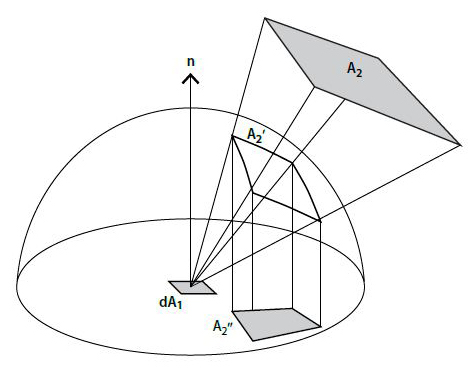
\includegraphics[width=0.55\linewidth]{assets/nusselt}
	\captionof{figure}{La analogía de Nusslet}
	\label{img:nusselt}
\end{figure}

El cálculo de la matriz de factores de forma $\mathbf{F}$ supone la proyección de los parches. De aquí en más se asumirá que estos parches son polígonos no curvos, lo que permite utilizar las técnicas de dibujado de objetos tridimensionales tradicionales como en la rasterización.

\subsubsection{Rasterización}
\label{sec:rasterizacion}

El <<\textit{rendering pipeline}>> es un proceso de dibujado estandarizado que consiste en un conjunto de etapas cuyo cometido es la generación de un \textit{frame buffer}. Los fabricantes de los dispositivos aceleradores gráficos y/o sistemas operativos proveen de interfaces de programación (OpenGL, Vulkan, DirectX) que se basan en este modelo para abstraer el uso del hardware.

Si bien el <<\textit{rendering pipeline}>> es modificable, cada una de sus etapas están definidas.  El programador es capaz de modificar pequeñas funciones (también llamadas \textit{kernels} o \textit{shaders}) que son ejecutadas en la GPU en las etapas correspondientes. El cometido de estas funciones es procesar los parámetros de entrada para generar parámetros que recibirá la siguiente etapa, que los recibirá y transformará como corresponda.

A continuación, se describe el proceso para OpenGL 4.5 visualizado en la Figura \ref{img:pipelinegl}, aunque muchas de estas etapas son trasladables a otras tecnologías existentes.

\vspace{5mm}
\begin{figure}[htbp]
	\centering
	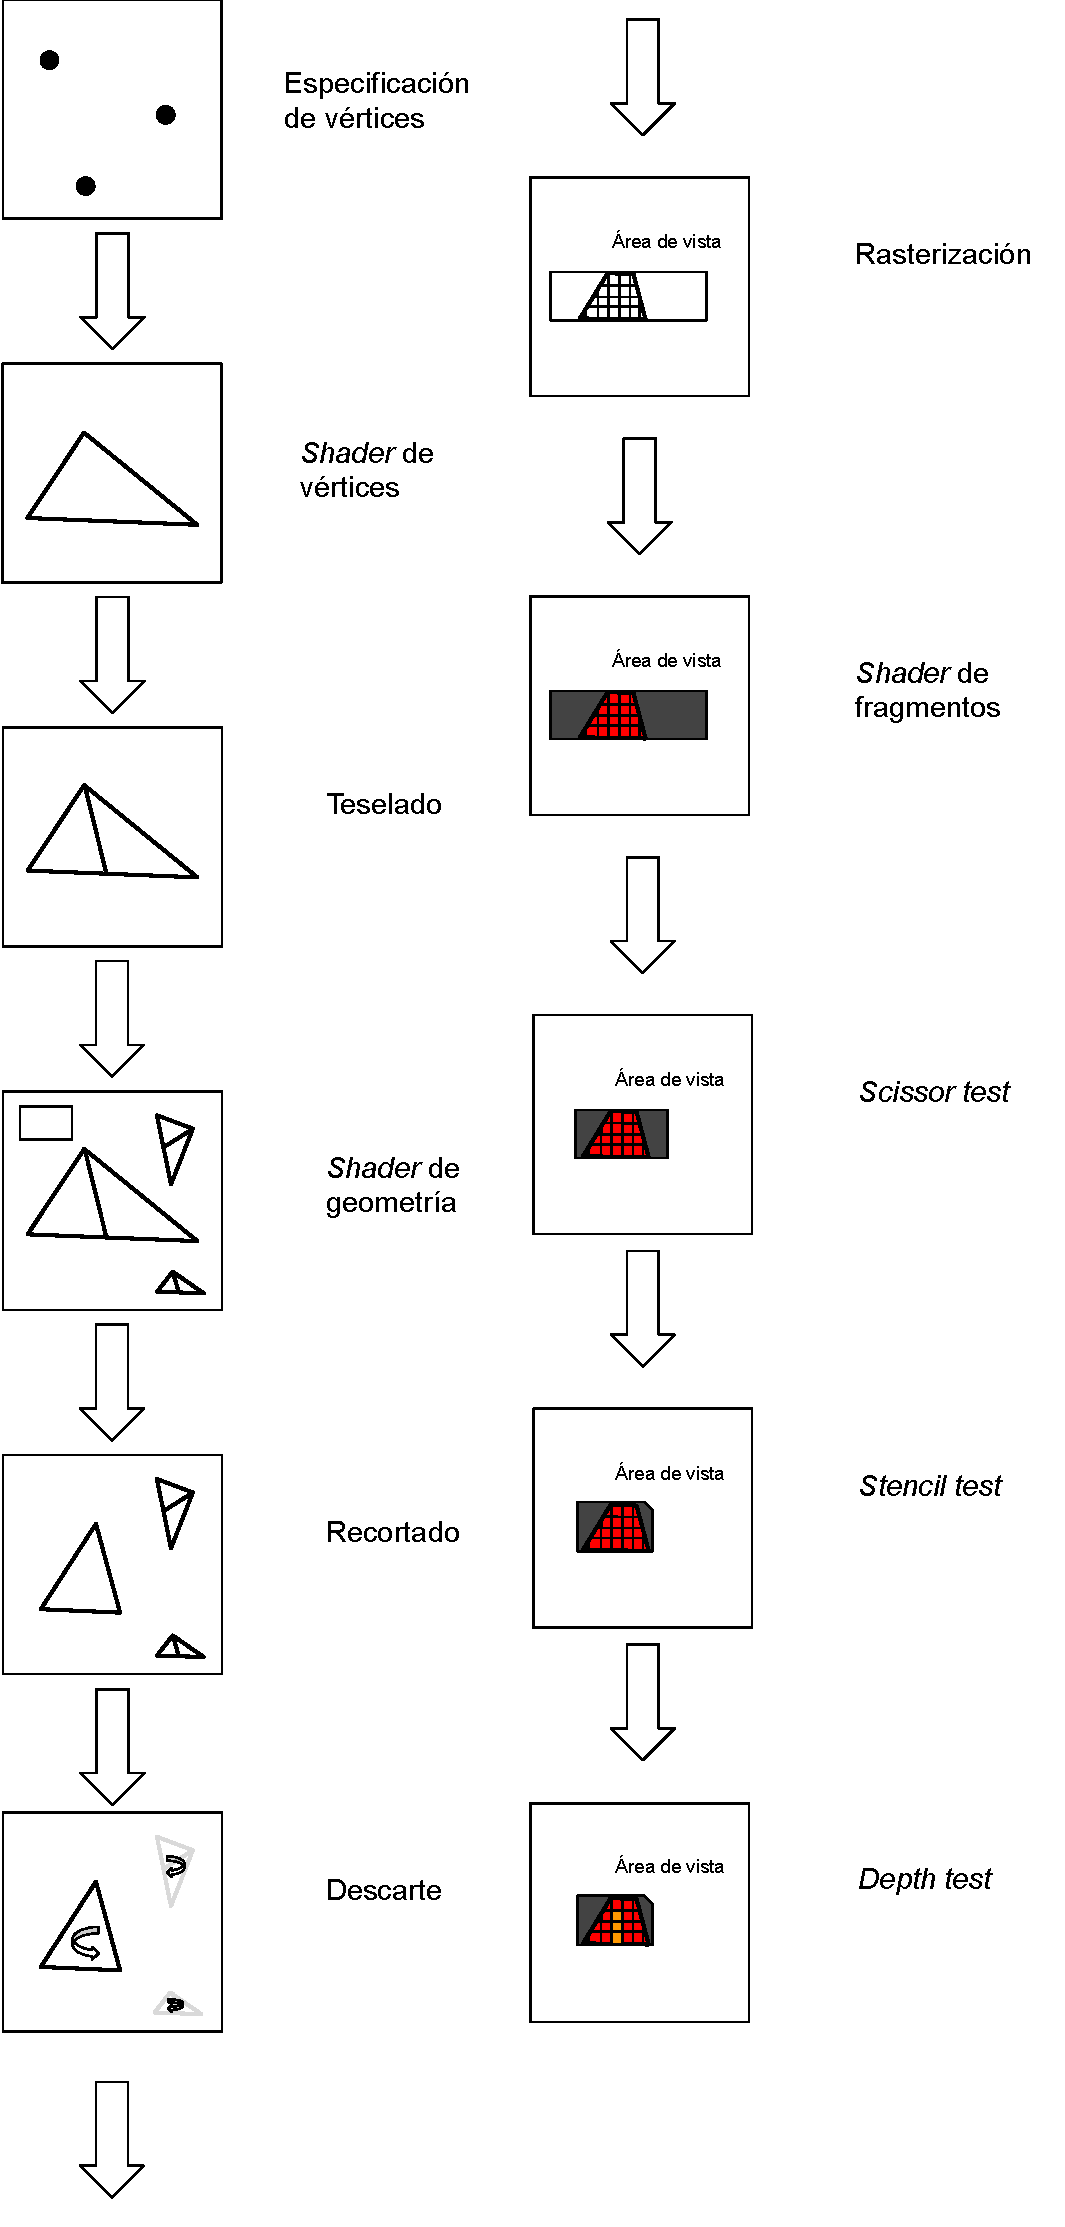
\includegraphics[width=0.55\linewidth]{assets/OpenGL}
	\captionof{figure}{El \textit{rendering pipeline} de OpenGL}
	\label{img:pipelinegl}
\end{figure}

\begin{enumerate}
	\item Procesamiento de primitivas geométricas:
		\begin{enumerate}
			\item Especificación de vértices: Inicialmente, las aplicaciones indican un conjunto de vértices a dibujar, definiendo cierto conjunto de primitivas geométricas como triángulos, cuadriláteros, puntos, líneas u otros.
			\item \textit{Shader de vétices}: Esta etapa transforma los vértices de entrada suministrados por la aplicación. Generalmente se computan las transformaciones lineales necesarias para cambiar la base de las coordenadas de los vértices de un sistema local al sistema global que defina la aplicación. Las coordenadas retornadas deberán corresponderse con coordenadas del espacio de recorte. Es decir, coordenadas correspondientes al volumen de vista.
			\item Teselado: En esta etapa se procesan los vértices a nivel de primitiva geométrica, con el objetivo de subdividirlas para mejorar la resolución obtenida.
			\item \textit{Shader de geometría}: En esta etapa también se procesan los vértices a nivel de primitiva geométrica con el objetivo de mutarlas y replicarlas.
			\item Recortado: Esta etapa es \textit{fija}, es decir, no es programable. Todas las primitivas calculadas anteriormente que residan fuera del volumen de vista serán descartadas en las etapas futuras. Además, se transforma las primitivas a coordenadas de espacio de ventana.
			\item Descarte: El proceso de descarte (en inglés \textit{culling}), es también fijo. Consiste en la eliminación de primitivas que no cumplan ciertas condiciones, como por ejemplo el descarte de caras cuya normal tiene dirección opuesta a la del observador.
		\end{enumerate}
	\item Procesamiento de fragmentos (rasterización):
		\begin{enumerate}
			\item Rasterización: El proceso de rasterización discretiza las primitivas en espacio de pantalla en un conjunto de fragmentos.
			\item \textit{Shader de fragmentos}: El procesamiento de cada fragmento se realiza a través del \textit{shader de fragmentos} que calcula uno o más colores, un valor de profundidad, y valores de plantilla (del inglés \textit{stencil}).
			\item \textit{Scissor test}: Todos los fragmentos fuera de un área rectangular definida por la aplicación son descartados.
			\item \textit{Stencil test}: Los fragmentos que no pasan la función de planilla definida por la aplicación no son dibujados, por ejemplo, simular el \textit{scissor test} que requieran primitivas más complejas.
			\item \textit{Depth test}: En esta etapa se ejecuta el algoritmo del Z-Buffer, donde sólo se escribirá el resultado en el \textit{frame buffer} de aquellos fragmentos que tengan la menor profundidad. Es decir, los que se encuentren más cerca del observador.
		\end{enumerate}
\end{enumerate}

Esta técnica de dibujado es extremadamente rápida, además, la mayoría de dispositivos contienen hardware especializado capaz de acelerar estos cálculos, comúnmente conocidos como Unidades de Procesamiento Gráfico (o GPU por sus siglas en inglés).

Con el objetivo de calcular los factores de forma utilizando este hardware Cohen y Greenberg \cite{Cohen} idearon el método del hemi-cubo.

\subsubsection{El método del hemi-cubo}

El hardware optimizado para realizar operaciones de rasterización tiene la capacidad de proyectar escenas tridimensionales sobre ventanas de vista planas a gran velocidad. 

El método original de cálculo de factores de forma propone la proyección de la escena sobre un hemisferio centrado en $S_{i}$, sin embargo los modelos de proyección utilizados no lo facilitan pues las proyecciones se realizan sobre superficies planas. Por esto, Cohen y Greenberg \cite{Cohen} proponen proyectar la escena a un hemi-cubo centrado en $S_{i}$, esto supone el dibujado de cinco superficies planas, y por tanto puede ser realizada utilizando la rasterización como se aprecia en la Figura \ref{img:ff3}.

Para utilizar el hardware eficientemente se considera que se calcula una fila completa de $\mathbf{F}$, esto implica que dado el parche $S_{i}$, se calcula simultáneamente los factores de forma desde $S_{i}$ al resto de las superficies restantes. 

Este método aprovecha el buffer de profundidad (Z-buffer), para la correcta determinación de visibilidad entre parches tomando en cuenta los fragmentos proyectados para los elementos que se encuentren más cercanos al parche $S_{i}$.

Este algoritmo, propone rasterizar la escena tridimensional en cinco texturas correspondientes a las caras de un hemi-cubo. Para cada fragmento renderizado se sumará un valor diferencial del factor de forma (o delta factor de forma), que dependerá de la posición del píxel en el hemi-cubo en relación a el hemisferio que este aproxima.  Esta suma genera una fila de la matriz $\mathbf{F}$, específicamente la fila $\mathbf{F}_{i}$, como se puede observar en la Eq. \eqref{eq:ffgreenberg}.

Por tanto, podremos definir:

\begin{equation}
	\mathbf{F}_{ij} = \sum_{q_{j}=1}^{R_{j}} \delta{F_{q_{j}}}
	\label{eq:ffgreenberg}
\end{equation}
donde:
\begin{itemize}
	\item $R_{j}$ es la cantidad de píxeles correspondientes a la superficie $S_{j}$ que cubren el hemi-cubo.
	\item $\delta{F_{q_{j}}}$ el delta factor de forma asociado al píxel del hemi-cubo $q_{j}$.
\end{itemize}

\vspace{5mm}
\begin{figure}[htbp]
	\centering
	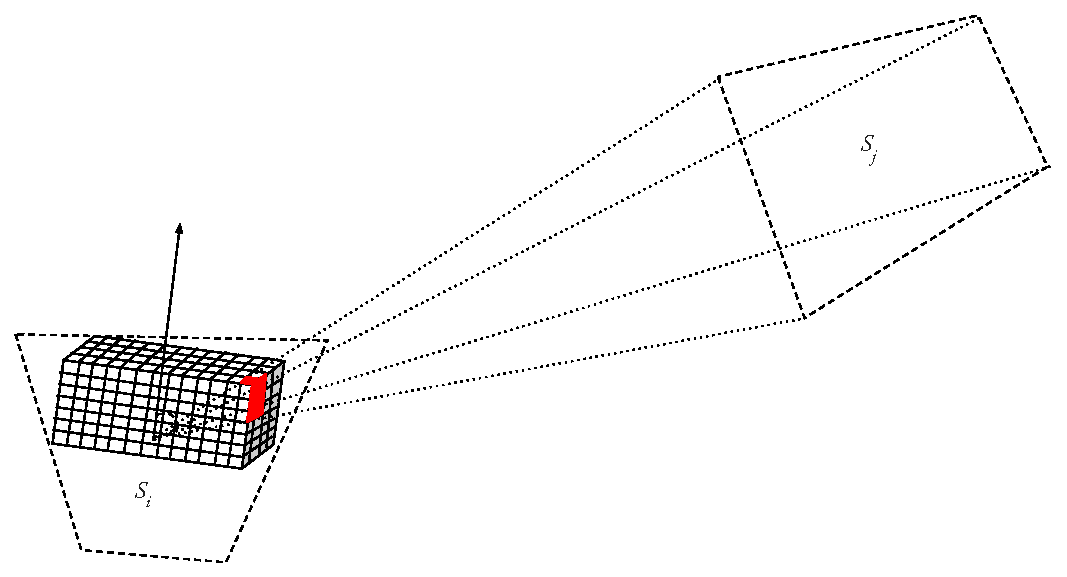
\includegraphics[width=0.8\linewidth]{assets/Hemicube}
	\captionof{figure}{Representación gráfica del método del hemi-cubo.}
	\label{img:ff3}
\end{figure}

Los delta factores de forma deben corregir la deformación introducida con el cambio de proyección desde un hemisferio a un hemi-cubo. Para ello, para cada píxel que compone el hemi-cubo es necesario calcular la proporción de área que este término ocupa en el hemisferio unitario.

Para la cara superior, los diferenciales se calculan como (ver referencias en la Figura \ref{img:deltaff}):

\begin{equation}
	\delta{F_{q}} = \frac{\cos{\phi_{i}}\cos{\phi_{j}}}{\pi{r^{2}}} \delta{A} = \frac{\delta{A}}{\pi({x^{2} + y^{2} + 1})} 
\end{equation}

Para las caras laterales, la fórmula dada es:

\begin{equation}
\delta{F_{q}} = \frac{\cos{\phi_{i}}\cos{\phi_{j}}}{\pi{r^{2}}}\delta{A} = \frac{z\delta{A}}{\pi({x^{2} + z^{2} + 1})}
\end{equation}

\begin{figure}[htbp]
	\centering
	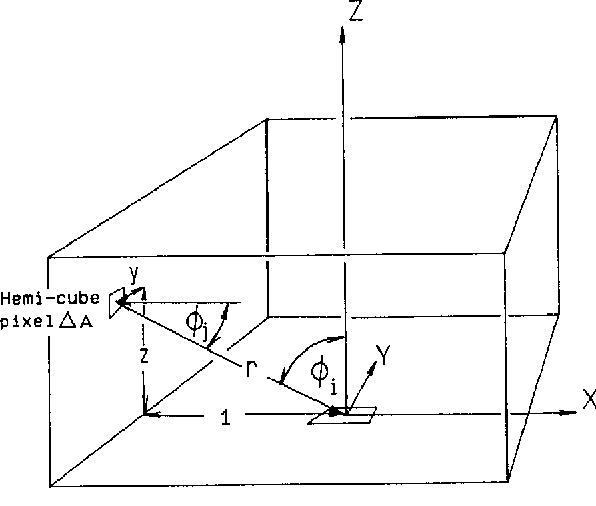
\includegraphics[width=0.4\linewidth]{assets/hemicube1}
	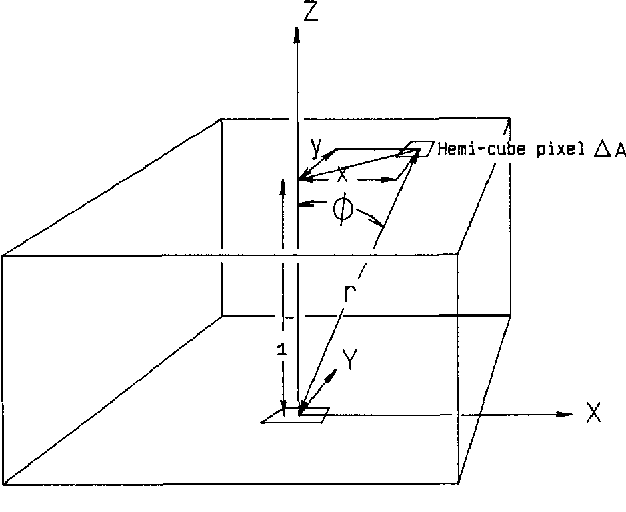
\includegraphics[width=0.4\linewidth]{assets/hemicube2}
	\captionof{figure}{Representación gráfica de los ejes considerados para el factor de corrección de los factores de forma. \cite{Cohen}}
	\label{img:deltaff}
\end{figure}


\subsubsection{Trazado de rayos}
\label{sec:raytracing}

Otra de las técnicas de simulación de iluminación existente es el ray tracing que consiste en el cálculo de la intersección de una semi-recta (a la que denominaremos rayo) con la geometría de la escena. Cada uno de estos rayos simulará un haz de luz.

Para cada uno de los rayos emitidos, se determinará el punto de intersección más cercano. Dada la primitiva geométrica interceptada, es posible integrar el resultado intermedio al resultado final, dependiendo del modelo de iluminación utilizado.

\subsubsection{El método del hemisferio}

El trazado de rayos es una técnica efectiva según Kajiya \cite{Kajiya}, para resolver la ecuación del rendering, utilizando la técnica de \textit{trazado de camino} donde el haz de luz absorbe las propiedades de los materiales con los que interactúa. En este algoritmo, la integral se resuelve con un método de Monte Carlo, donde cada rayo representa una muestra estadísticamente independiente. Para resolver la doble integral presentada en la Eq. \eqref{eq:ff}.

Es posible pensar el problema original colocando un hemisferio unitario en el centro de $S_{i}$ orientada en la dirección de la normal de la superficie.

El algoritmo propuesto por \citeauthor{Malley} \cite{Malley} consiste realizar un muestreo de la cantidad de  rayos que parten desde el centro de $S_{i}$ e intersecan $S_{j}$. Las direcciones de los rayos serán determinadas a partir de la \textit{distribución del coseno} cuya función de densidad es $f(x) = \frac{1}{2}[1 + \cos((x-1)\pi)]$ donde $x$ es una variable aleatoria uniforme en el rango $[0,1]$.

\begin{equation}
	\mathbf{F}_{ij} = \frac{1}{nMuestras} \sum_{k=1}^{nMuestras} {\beta(ray(S_{i},d), S_{j})}
	\label{eq:ffhemiesfera}
\end{equation}
donde: \begin{itemize}
		\item  $d$ sigue la distribución coseno.
		\item $\beta(r, S_{j})$ toma el valor 1 si el rayo $ray(S_{i},d)$ interseca a $S_{j}$ o $0$ en otro caso.
	   \end{itemize}
\clearpage

\vspace{5mm}
\begin{figure}[htbp]
	\centering
	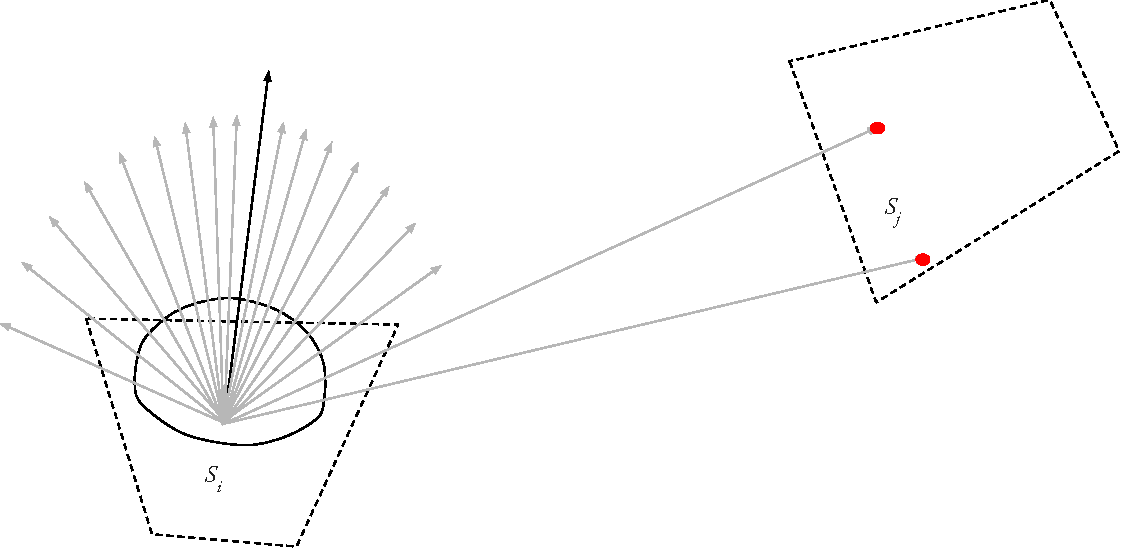
\includegraphics[width=\linewidth]{assets/Raytracing}
	\captionof{figure}{Representación gráfica del método de método de trazado de rayos para el cálculo de factores de forma}
	\label{img:ff}
\end{figure}

Cabe destacar que no es necesario utilizar una distribución de probabilidad con valores aleatorios o pseudo-aleatorios, sino que alcanza con utilizar una secuencia determinista de rayos que tengan una distribución que siga la del coseno.

Para esto, pueden utilizarse otras distribuciones para la dirección de traza. Particularmente, una de ellas es la propuesta por Beckers y Beckers \cite{Beckers}, que presentan un método general de teselación de discos y hemisferios. Es deseable el hecho de que la propuesta para hemisferios genera un conjunto de celdas de igual factor de forma, es decir, las celdas del disco proyectado tienen la misma área. Esto hace que el método presente una calidad adecuada para la elección de las direcciones en la que se trazarán los rayos.

\subsection{Extensión a superficies especulares}

Originalmente, el método de cálculo de la radiosidad asume que todas las superficies son reflectores lambertianos, lo que supone que solo existirán reflexiones difusas cuando la luz interactúa con ellas. Sin embargo, en la mayor parte de las escenas del mundo real es necesario simular reflexiones especulares correctamente para obtener resultados que se asemejen a la realidad.

Por ello se ha desarrollado una extensión del método de radiosidad para superficies especulares o refractantes propuesto por Sillion, et al \cite{Sillion}. Los autores proponen extender el significado del término \textit{factor de forma} a más que una mera relación geométrica entre parches. El nuevo factor de forma $\mathbf{F}_{ij}$ corresponde a la proporción de luz que sale de la superficie $i$ y llega la superficie $j$ luego de un número de reflexiones y refracciones especulares. Esta propuesta modifica completamente los algoritmos de cálculo de factores de forma. Los autores proponen un algoritmo de cálculo que consiste en el trazado de caminos desde $S_{i}$ en una dirección arbitraria $d$ bien distribuida.  Luego, para cada camino trazado, se distribuirá el valor final del factor de forma dependiendo en la cantidad de superficies con las que interaccione el camino y sus coeficientes especulares como se observa en la Figura \ref{img:caminoespecular}.

\vspace{5mm}
\begin{figure}[htbp!]
	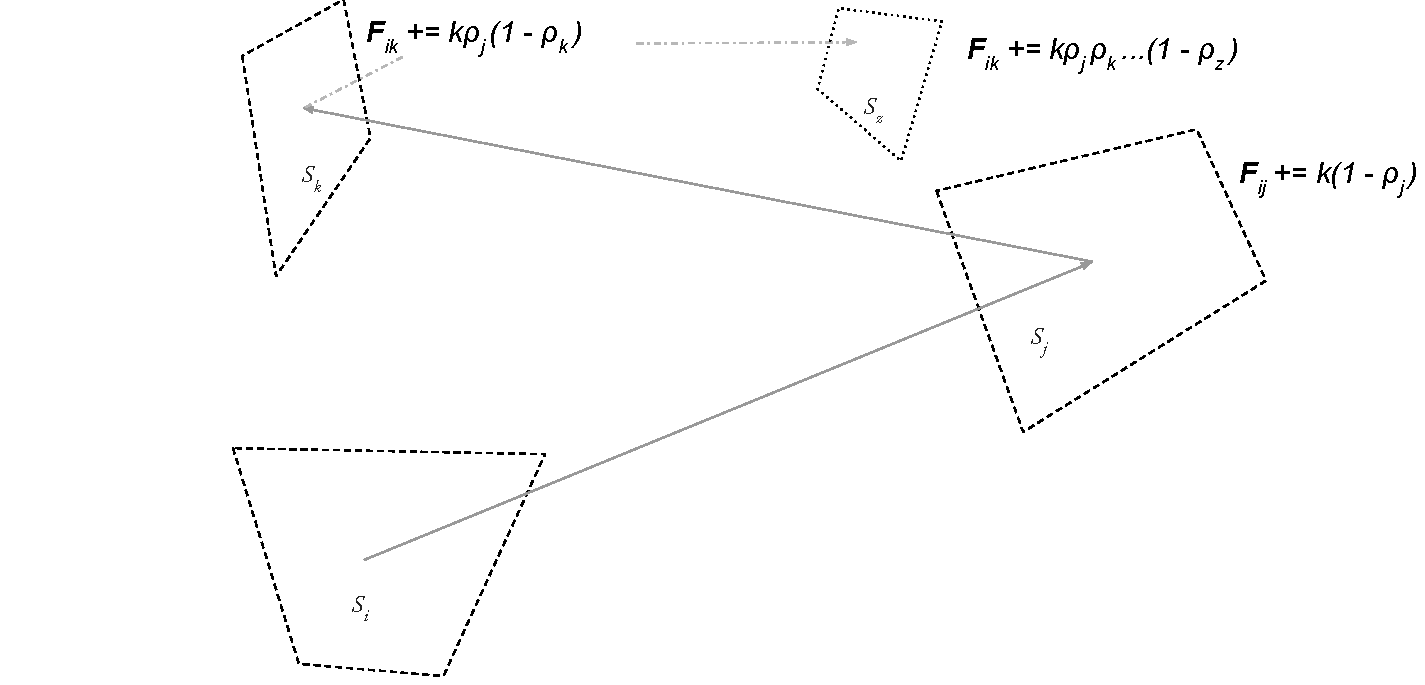
\includegraphics[width=1\linewidth]{assets/extended}
	\captionof{figure}{Representación gráfica del cálculo del factor de forma extendido donde $k = \frac{1}{N}$, con $N$ muestras tomadas.}
	\label{img:caminoespecular}
\end{figure}

Este método supone el trazado de rayos recursivo. En primer lugar, se lanza un rayo desde la superficie $S_{i}$, si  interseca una cara cuyo coeficiente de reflexión especular es mayor a cero se almacenará el total de $k(1 - \rho^{(s)}_{j})$ (donde $k = \frac{1}{nMuestras}$) como contribuyente del factor de forma $\mathbf{F}_{ij}$ y se calcularán las siguientes intersecciones con el residuo de la reflexión que se distribuirá entre los parches reflejados. Es decir, suponiendo que un rayo impacta $S_{k}$ desde el camino $(S_{i}, S_{j})$ donde $\rho^{(d)}_{j} \ge 0$ se agregará $k\rho^{(d)}_{j}(1 - \rho^{(s)}_{k})$ y se procederá hasta que $\rho^{(s)}_{z} = 0$ para una superficie intersecada $S_{z}$ o se alcance el máximo límite de recursión. Cabe destacar, que para que el algoritmo correctamente represente la realidad, se debe respetar la relación $0 < \rho^{(d)}_{i} + \rho^{(s)}_{i} <= 1$.

\subsection{Cálculo del vector de radiosidades}
\label{sec:vrad}

Luego de computar la matriz $\mathbf{F}$ y dado los vectores de emisiones $E$ y reflexiones $R$, resta computar el vector de radiosidades correspondiente para cada parche, denominado $B$.

Recordando la Eq. \eqref{eq:radiosity}, es posible deducir el problema al sistema de ecuaciones dado por:

\begin{equation}
	E = (\mathbf{I} - \mathbf{RF})B
\end{equation}

Los estudios de álgebra lineal modernos permiten la resolución de sistemas de ecuaciones de forma optimizada, dependiendo de las propiedades observadas.

Recordando las propiedades en la Sección \ref{propsff}, podemos observar que:

\begin{itemize}
	\item $\sum_{j=1}^{N} \mathbf{F}_{ij} \leq 1 \forall{i \in [1,N]}$
	\item $\rho^{(d)}_{i} \leq 1 \rightarrow \sum_{j=1}^{N} \mathbf{R}_{ij} \leq 1 \forall{i \in [1,N]}$
\end{itemize}

Esto implica que las entradas de $\mathbf{RF}$ s\texttt{}on siempre menores a $1$, por tanto la matriz $(\mathbf{I} - \mathbf{RF}) = M$ es diagonal dominante ya que $\sum_{j=1}^{N}|R_{ij}F_{ij}| \le 1 \forall i \in [1, N]$ y $R_{ii}F_{ii} = 0  \forall  i \in [1,N]$. Esto garantiza la convergencia del uso de métodos de resolución iterativos o de factorización, como el algoritmo de Gauss-Seidel o la factorización LU.

Aunque los algoritmos clásicos de resolución de sistema de ecuaciones aplican a este problema, existen optimizaciones que hacen que su resolución se pueda aproximar de manera razonable con un costo computacional muy menor. Para ello, considerando que la matriz $\mathbf{F}$ es diagonal dominante, podemos utilizar la equación \ref{eq:iterativo} pues el \textit{residuo} (el término agregado en cada iteración) se reduce de la siguiente forma: $\left\|\mathbf{RF}B^{(i+1)}\right\| < \left\|\mathbf{RF}B^{(i)}\right\|$. El método planteado en la Eq. \eqref{eq:iterativo} es el método de Jacobi.

\begin{equation}
	B^{(i+1)}  = \mathbf{RF}B^{(i)}  + E \text{ con }  B^{(0)} = E
	\label{eq:iterativo}
\end{equation}

Cabe aclarar, que el método planteado hasta el momento resuelve la radiosidad en un único canal. Es decir, no se toma en cuenta todo el espectro electromagnético de la luz, es por ello que puede establecerse una extensión del método. Esta extensión implica la existencia de tres vectores de reflexión, uno para cada canal \textit{RGB} (del inglés \textit{Red - Green - Blue}). Por tanto es necesario que se resuelvan tres y no un único sistema de ecuaciones, aunque es posible destacar que la matriz $\mathbf{F}$ permanece constante pues depende únicamente de la geometría de la escena. El único cambio en el sistema surge en la matriz $\mathbf{R}$ que pasará a depender del canal seleccionado: $\mathbf{R}_{c}$.

\section{Bibliotecas gráficas}

La computación gráfica es una herramienta sumamente útil para la generación de programas que faciliten tareas. Es por ello que ha sido necesario proveer bibliotecas estándar capaces de facilitar la aplicación de técnicas como la rasterización o el trazado de rayos utilizando las aceleraciones por hardware disponibles y de forma abstracta. Es por esto que generalmente se utilizan bibliotecas gráficas que abstraigan el hardware subyacente para el programador.

\subsection{OpenGL}

Existen un conjunto bibliotecas de gráficas que soportan la rasterización (OpenGL, Vulkan, DirectX, Metal). En el contexto de este proyecto, se estudia el uso de Open Graphics Library (OpenGL).

OpenGL es una especificación de una Interfaz de Programación de Aplicación (API por sus siglas en inglés) diseñada por la organización Khronos Group. Su cometido es el dibujado de gráficos bidimensionales o tridimensionales utilizando el método de rasterización (ver Sección \ref{sec:rasterizacion}). Los distintos fabricantes de sistemas operativos y tarjetas gráficas proporcionan implementaciones que se ajusten al hardware específico. Esta abstracción facilita la compatibilidad de las aplicaciones independientemente del hardware donde sean ejecutadas.

\subsubsection{Arquitectura}
La arquitectura base de la biblioteca es de cliente/servidor (ver Figura \ref{img:gpucpugl}). El cliente es la aplicación que invoca funciones para el dibujado de gráficos y es ejecutado en la CPU. El servidor, que es ejecutado en la GPU, almacena los distintos buffers y ejecuta las funciones necesarias.

El cliente modifica los atributos a través de invocaciones a las funciones de prefijo \verb|gl|, identificando el recurso afectado con valores enumerados (por ejemplo, \verb|GL_TEXTURE_2D| representa un conjunto de texturas bidimencionales). Dado que la biblioteca es implementada como una máquina de estado, los atributos son recordados hasta que sean modificados nuevamente.

Estas invocaciones no son ejecutadas inmediatamente, sino que de forma similar a un buffer de entrada/salida son almacenados para ser ejecutados cuando sea necesario, es decir, cuando se requiera el dibujo de una nueva imagen. Esto hace que la ejecución de comandos sea asíncrona, y por tanto mejora el rendimiento previniendo la sincronización entre la CPU y GPU.

\vspace{5mm}
\begin{figure}[h]
	\centering
	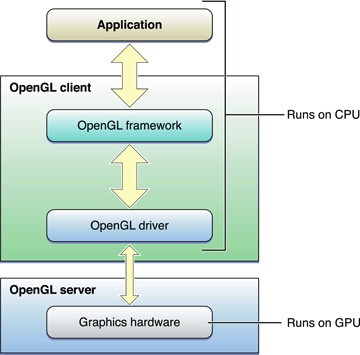
\includegraphics[width=.4\linewidth]{assets/cpu_gpu}
	\caption{Vista general de la arquitectura de OpenGL}
	\label{img:gpucpugl}
 \end{figure}

\subsubsection{Extensiones}
La inicialización de la máquina de estados depende directamente de la creación de un contexto que será utilizado para almacenar los datos. Este proceso depende fuertemente de la plataforma donde se ejecute la aplicación, que depende entre otros del sistema operativo y/o del hardware utilizado. Por este motivo, existen bibliotecas que manejan la creación del contexto en diversas plataformas como SDL y GLFW.
	
\subsection{Embree}

Los distintos algoritmos para evaluar la intersección entre superficies y rayos han evolucionado en los últimos años, introduciéndose los conceptos de volumen acotante y jerarquías de escena. Esto resulta en un gran trabajo innecesario al momento de implementar algoritmos que se basan en el trazado de rayos de forma eficiente. Es por ello, que de manera similar a las APIs de dibujado de gráficos acelerados por hardware existen interfaces que facilitan la aceleración del trazado de rayos. En particular, Embree es una biblioteca creada por Intel con este propósito.

Embree expone un conjunto de funciones para realizar el trazado de rayos acelerado a través de componentes de hardware y software mediante la utilización del conjunto de instrucciones del paradigma SIMD (del inglés Single Instruction - Multiple Data), donde una única instrucción es ejecutada sobre un gran conjunto de datos. Por ejemplo, la ejecución concurrente de un conjunto de multiplicaciones en punto flotante a nivel de CPU. Además posibilita la generación de estructuras de aceleración, como las BVH (del inglés \textit{Bounding Volume Hierarchies}). La arquitectura de la aplicación, diagramada en la Figura \ref{img:embree}, demuestra los distintos algoritmos propuestos para la generación de estructuras de aceleración y algoritmos de intersección eficientes.

La biblioteca resuelve un conjunto de dificultades normalmente encontradas en todas las aplicaciones de algoritmos que involucren el trazado de rayos, entre ellas:

\begin{itemize}
	\item \textbf{Multi-hilo:} Con el objetivo de ejecutar distintos kernels de traza de rayos de forma concurrente, la biblioteca provee de funciones \textit{thread-safe} para el dibujado y la generación de estructuras de aceleración.
	\item \textbf{Vectorización:} Con el objetivo de optimizar el uso de la CPU, la biblioteca vectoriza los cálculos necesarios para aprovechar las instrucciones SIMD.
	\item \textbf{Soporte para múltiples CPUs:} La biblioteca provee de una capa de abstracción independiente del hardware donde se utilice.
	\item \textbf{Conocimiento del dominio extenso:} Dado que la biblioteca implementa las estructuras de aceleración y los algoritmos de intersección no es necesario tener un conocimiento completo del dominio para construir aplicaciones utilizando trazado de rayos.
	\item \textbf{Manejo eficiente de la memoria:} Se provee un manejo interno de la memoria RAMo para facilitar la visualización de escenas con gran cantidad de primitivas.
\end{itemize}

\vspace{5mm}
\begin{figure}[H]
	\centering
	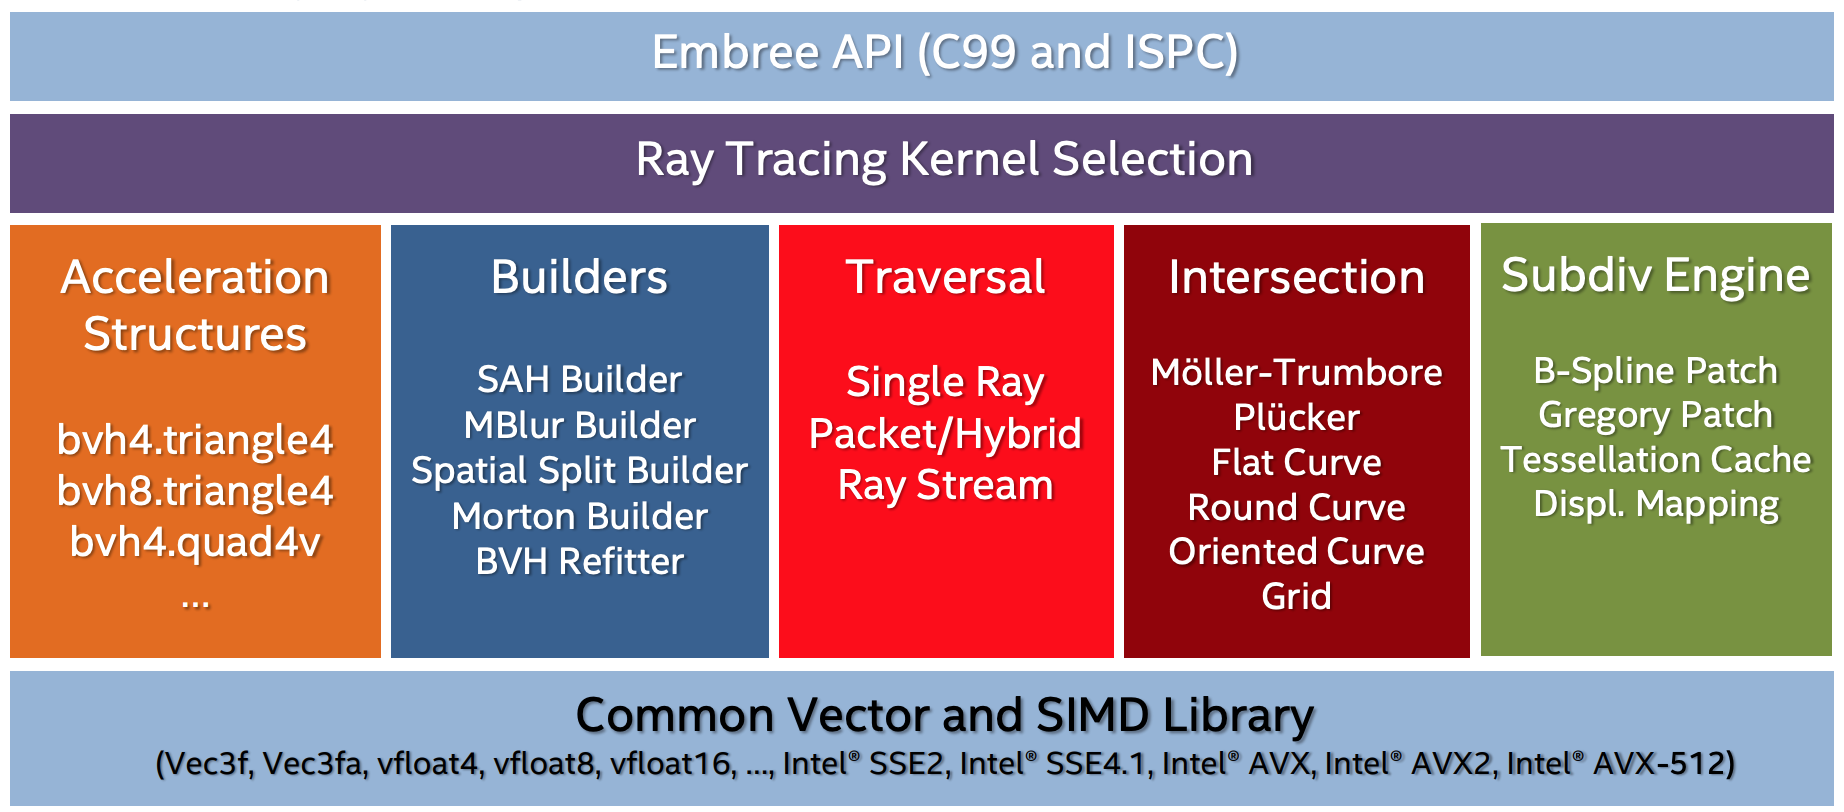
\includegraphics[width=.8\linewidth]{assets/embree}
	\caption{Vista general de la arquitectura de Embree}
	\label{img:embree}
\end{figure}

\section{Trabajos relacionados}

En esta sección se discuten alternativas propuestas para resolver el cálculo de la iluminación global en escenas con materiales difusos y especulares.

El algoritmo propuesto por Shirley \cite{Shirley} calcula la iluminación difusa utilizando dos pasadas. Este algoritmo difiere del propuesto por Sillion y Puech \cite{Sillion} en el sentido que se consideran distintos modelos de fuentes luminosas con propiedades particulares (luces puntuales, direccionales, de área).

En la primer pasada, el algoritmo calcula la componente difusa de todos los rayos que rebotan en al menos una superficie especular. Este método calcula los caminos que seguirán los rayos de luz provenientes de fuentes luminosas, es decir, se discretiza la cantidad de rayos emitidos por una fuente luminosa, cada rayo representa una fracción de la energía emitida.

Cuando existe una intersección, se divide la energía entre los cuatro nodos más cercanos (estos nodos almacenan la radiosidad) a través de una estimación para calcular qué área ocupa cada uno de ellos, de esta manera es posible generar un mapa de radiosidad para la superficie. Dado que la iluminación directa (es decir, aquellos rayos que no se intersecan con superficies especulares) es calculada en la etapa de vista, solo es necesario computar los rebotes especulares, para ello se traza un número bajo de rayos distribuidos de forma uniforme para encontrar las zonas donde existan superficies especulares, luego se trazan rayos en esa dirección de forma "densa", que implica trazar una cantidad de rayos considerable en una dirección que no varía demasiado.

El segundo paso utiliza el método de radiosidad para calcular la iluminación difusa que involucra al menos dos superficies, nuevamente se omite la iluminación directa pues se calculará en la etapa de vista. Para ello, se emiten rayos desde cada superficie utilizando la distribución del coseno de manera equivalente a la propuesta por \citeauthor{Malley}. 

Finalmente, cuando se dibuja la imagen final también se calcula la iluminación directa de forma estándar (ver Whitted \cite{Whitted}) sustituyendo el término de ambiente por el calculado en las pasadas anteriores.

Otro acercamiento al problema es el método propuesto de Kok \cite{Kok} es una extensión para parches que están formados por superficies de Bézier, estas son superficies delimitadas por curvas de nombre homónimo que para una superficie definida con $m$ puntos siguen la ecuación $c(u,v) = \sum_{i=0}^{m} c_{i}(v)B_{i}^{m}(u)$ donde $c$ es el vector de desplazamientos, y $B$ una función que genera la curva.

Los autores proponen la discretización de las superficies en puntos de muestreo dependiendo del área, luego simplemente se calcula el factor de forma de la superficie utilizando el método del hemisferio, agregando los resultados para cada punto. En caso de que un rayo intersecta una superficie especular, los autores proponen un método similar al de Sillion y Puech \cite{Sillion} donde se seguirá el camino del rayo mientras rebote en superficies especulares y arribe en una difusa, distribuyendo el factor de forma entre las superficies involucradas dependiendo del coeficiente de reflexión especular.

Una formulación distinta del problema, que también se focaliza en el uso de radiosidad es Holly y Torrance \cite{Holly}. Los autores proponen, nuevamente, un método de dos pasadas donde el factor de forma está compuesto por tres partes, el factor de forma difuso y los factores de forma delantero y trasero. El primero, está intrínsecamente relacionado a la reflexión difusa y tiene el mismo comportamiento que el factor de forma definido por Cohen \cite{Cohen} mientras que los segundos se relacionan con el fenómeno de la refracción y son calculados integrando en el hemisferio opuesto por la normal del parche. La última componente son los factores de forma de ventana, que contienen la información referente a la reflexión especular.

El método propone el uso del hemi-cubo para calcular los factores de forma delanteros, mientras que los traseros son calculados invirtiendo el hemi-cubo. Para calcular las componentes especulares, se utiliza un método comúnmente denominado dibujado de portales, donde se coloca una ventana virtual que distorsiona la proyección de la escena al mover la cámara, con la salvedad de que se opta por duplicar la geometría simétricamente en lugar de simplemente trasladar la cámara.